\section{Instrumentation}
I don't think there's much we need to know here (if anything at all), 
but I'm adding a few things that shouldn't be hard to study and might come up.  

\subsection{Questions}
\begin{enumerate}
\item \textbf{Describe quantitatively the point spread function of a diffraction-limited optical
      telescope. Explain how diffraction spikes arise, and what determines their positions
      and intensities. Under what circumstances will the PSF be broadened by atmospheric
      turbulence?}
\item \textbf{Derive an expression for the point source sensitivity of a radio interferometer as
      a function of the frequency, bandwidth, system temperature, diameter of each dish,
      number of dishes, etc.}

      \newthought{Let's begin by} deriving the point source sensitivity of a single dish
      radio telescope.  To do so, we need a little bit of background on what a radio telescope
      is.  There are two broad classes of single-dish radio telescopes: those with coherent
      detectors and those with incoherent detectors.  Coherent detectors measure the amplitude
      and phase of the incoming electric field, while incoherent detectors discard the phase
      information.  In this way, incoherent detectors are essentially very sensitive thermometers.
      We will focus this discussion on coherent detectors (because the phase information is needed
      for interferometry).

      A radio telescope can be broken down into a number of parts.  We will consider these
      parts in the order that they translate the sky brightness into a brightness temperature.
      \begin{itemize}
      \item The antenna and feed

            First, there must be a component that is sensitive to a time varying electric
            field.  The feed converts the time varying electric field into a time varying voltage.
            This can be a massive dish with a feed at its focus, or merely a
            simple piece of wire acting as a dipole antenna.  Obviously the large dish will
            be very sensitive in the forward direction, while the simple dipole antenna will
            be sensitive to almost the entire sky, but not particularly sensitive in any one
            direction.  The pattern of sensitivity for an antenna is called its ``gain pattern''.
            The higher the gain in a given direction, the more sensitive the antenna is to signals
            from that direction.  This gain pattern is typically encoded in the ``effective
            collecting area'' of the antenna.

            It can be shown that for any antenna the angle-averaged effective collecting area
            is given by
            \begin{dmath}\label{eq:Ae}
                \langle A_e\rangle = \frac{\lambda^2}{4\pi}
            \end{dmath},
            where $\lambda$ is roughly the central wavelength of the bandpass.  We can get
            an intuitive understanding for why this equation must be true by comparing the
            100 m Green Bank telescope with a simple LWA dipole.  The Green Bank telescope
            has a $\pi(50~{\rm m})^2 \approx 8000~{\rm m}^2$ collecting area in its forward
            direction, and a low (but nonzero) sensitivity in the off-axis directions coming
            in through the telescope's sidelobes.  Averaging over all angles reproduces
            Equation~\ref{eq:Ae}.  On the other hand, the LWA dipoles are roughly evenly
            sensitive to the whole sky.  Therefore, at $\lambda=10~{\rm m}$ each dipole has
            an effective collecting area of $\approx 8~{\rm m}^2$ towards all parts of the sky.

            Finally, it should be noted that an antenna can only be sensitive to one polarization
            of light.  Therefore, in order to measure the total power from a source one must
            build two feeds so that one is sensitive to each polarization.

      \item The receiver

            The receiver is a general term for the electronics that process the signal coming
            from the feed.  For a radiometer\sidenote{
                A radiometer simply measures the total power in the voltage fluctuations coming
                from the feed.
            }, the receiver will consist of (in its simplest design):
            a gain stage to amplify the signal,
            a bandpass filter to restrict the signal to a known frequency range,
            a square law detector that produces a voltage output proportional to the total
            power\sidenote{
                $V_{\rm out} \propto V_{\rm in}^2$
            }, and an integrator that accumulates the voltage samples over a given time.

            Additionally, most radiometers include electronics to stabilize the gain of the
            amplifiers, analog to digital converters that sample and digitize the signal\sidenote{
                Digital signals are less likely to deteriorate as they pass through lossy cable.
                However the digitization process itself is lossy and can restrict the dynamic
                range of the telescope if not enough bits are used to represent the signal.
                The rate at which an ADC must sample is determined by the Nyquist frequency.
            }, and a mixer that converts high frequency signals into low frequency signals
            that are easier to process electronically.
      \end{itemize}

      Now let's assume we have an antenna with a bandwidth $B$ (set by the bandpass filter),
      integration time $\tau$.  After the integrator we have an estimate for the system
      temperature $T_{\rm sys} = P_\nu/k$, where $P_\nu$ is the power per unit frequency in the
      antenna and $k$ is the Boltzmann constant.  With an ADC sampling at the Nyquist frequency,
      the integrator uses $2B\tau$ independent samples of the power to estimate $T_{\rm sys}$.
      Therefore, the uncertainty on the measurement of $T_{\rm sys}$ is
      \begin{dmath*}
        \sigma_T = \frac{\sigma_{T,0}}{\sqrt{2B\tau}}
      \end{dmath*},
      where $\sigma_{T,0}$ is the uncertainty on a single sample of $T_{\rm sys}$.  To derive
      $\sigma_{T,0}$ we use the fact that $T_{\rm sys} \propto \langle V^2\rangle$ where $V$
      is the voltage before the square-law detector.  Setting the constant of proportionality
      to unity we have
      \begin{dmath*}
        \sigma_{T,0}^2 = \langle V^4\rangle - \langle V^2\rangle^2
                       = \frac{1}{\sqrt{2\pi T_{\rm sys}}}\int_{-\infty}^{+\infty} V^4e^{-V^2/2T_{\rm sys}}\,\d V
                       - \left(\frac{1}{\sqrt{2\pi T_{\rm sys}}}\int_{-\infty}^{+\infty} V^2e^{-V^2/2T_{\rm sys}}\,\d V\right)^2
                       = 3T_{\rm sys}^2 - T_{\rm sys}^2 \nolinebreak = 2T_{\rm sys}^2
      \end{dmath*}.

      Finally, we want to relate the measured system temperature with the observed flux $S$.
      The system temperature is a combination of many components, only one of which is the
      astrophysical signal we are interested in:
      \begin{dmath}
        T_{\rm sys} = T_{\rm signal} + T_{\rm noise} + T_{\rm atmosphere} + \cdots
      \end{dmath}.
      In the limit where $T_{\rm signal} \ll T_{\rm sys}$, the uncertainty on $T_{\rm signal}$
      is dominated by the uncertainty on $T_{\rm sys}$, which we have already derived.
      Finally we can relate $T_{\rm signal}$ to the observed flux by remembering that each
      antenna is only sensitive to one polarization and hence can only detect half the flux:
      \begin{dmath}
        kT_{\rm signal} = \frac{SA_e}{2}
      \end{dmath},
      where $A_e$ is again the effective collecting area.

      Therefore we have derived the radiometer equation, which describes the temperature
      sensitivity of a single dish radio telescope (in the absence of gain fluctuations in
      the amplification stage of the receiver):
      \begin{dmath}\boxed{
        \sigma_S = \frac{2kT_{\rm sys}}{A_e\sqrt{B\tau}}
      }\end{dmath}

      For an interferometer, we replace the square-law detector with a correlator that multiplies
      voltages from different antennas.  In that case
      \begin{dmath*}
        \sigma_{T,0}^2 = \langle V_i^2V_j^2\rangle - \langle V_iV_j\rangle^2
                       = \langle V_i^2\rangle\langle V_j^2\rangle \nolinebreak
                       = T_{\rm sys}^2
      \end{dmath*},
      so for a two-element interferometer we have
      \begin{dmath}
        \sigma_S = \frac{\sqrt{2}kT_{\rm sys}}{A_e\sqrt{B\tau}}
      \end{dmath}.
      In an array with $N$ antennas there are $N(N-1)/2$ baselines (pairs of antennas).
      Each baseline represents an independent measurement of the flux\sidenote{
        If you disagree with this, like me, there are apparently some subtleties that make
        each baseline independent from the others.  I've spent the better part of a few months
        trying to understand this and I don't think I'm there yet.

        --Michael
      }, therefore
      \begin{dmath}\boxed{
        \sigma_S = \frac{2kT_{\rm sys}}{A_e\sqrt{N(N-1)B\tau}}
      }\end{dmath}.

\item \textbf{Describe some of the common technologies for detecting gamma rays, the approximate
      energy range over which they are applicable, and some of their main advantages
      and disadvantages.}
\end{enumerate}


\subsection{Telescope Design}
Here's a diagram of a telescope, with the focuses labeled.  There's also the 
prime focus (at the position of the secondary mirror) and the coude focus 
(the light is sent into another room with really big instruments).  

\begin{figure}[!h]
\begin{center}
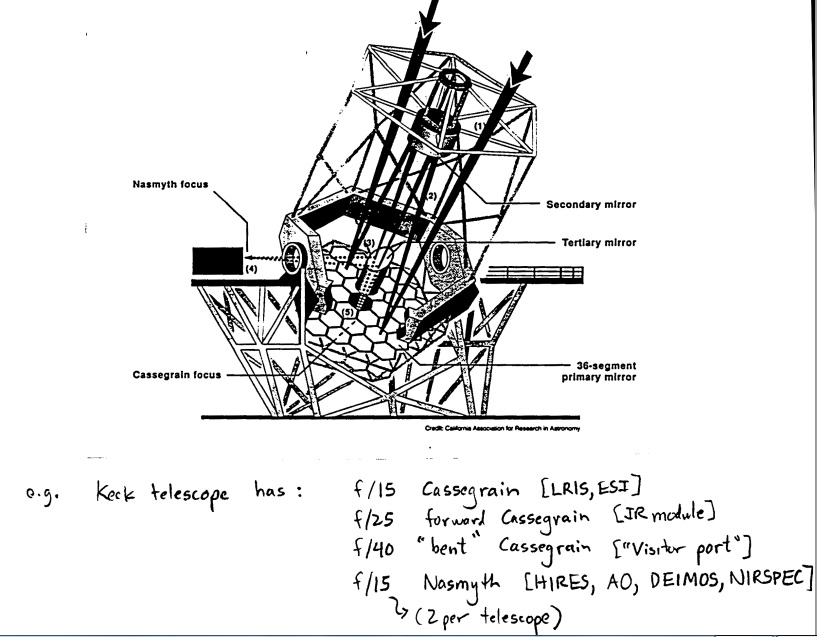
\includegraphics[width=\textwidth]{telescope.jpg}
\end{center}
\caption{Make sure it's pointed up.
\label{fig:telescope}}
\end{figure}

\subsection{Spectrographs}
Here's a basic spectrograph layout.  Also possibly useful- in an echelle 
spectrograph, the light is dispersed twice, onto a two dimensional plane.  
The first dispersion separates the light into different wavelengths, but 
the different diffraction orders overlap.  A second disperser splits the 
orders in the other direction.  The result is the wavelength changes from 
left to right across the orders, and the orders (different wavelength ranges) 
change from top to bottom.  

\begin{figure}[!h]
\begin{center}
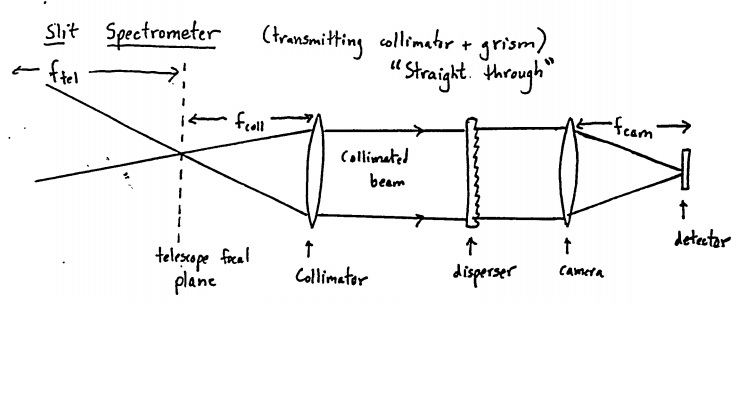
\includegraphics[width=\textwidth]{spectrograph.jpg}
\end{center}
\caption{Double rainbow!  All the way across the focal plane!.
\label{fig:spectrograph}}
\end{figure}


\subsection{CCDs}
Photons hitting a CCD remove electrons from the atoms in the CCD.  These 
electrons are trapped below the photon collecting later in a potential well, 
then changing voltages move the electrons to the edge, then corner of the 
CCD where the number of electrons can be measured, corresponding to which 
pixels were hit by photons.  Here's the basic idea:

\begin{figure}[!h]
\begin{center}
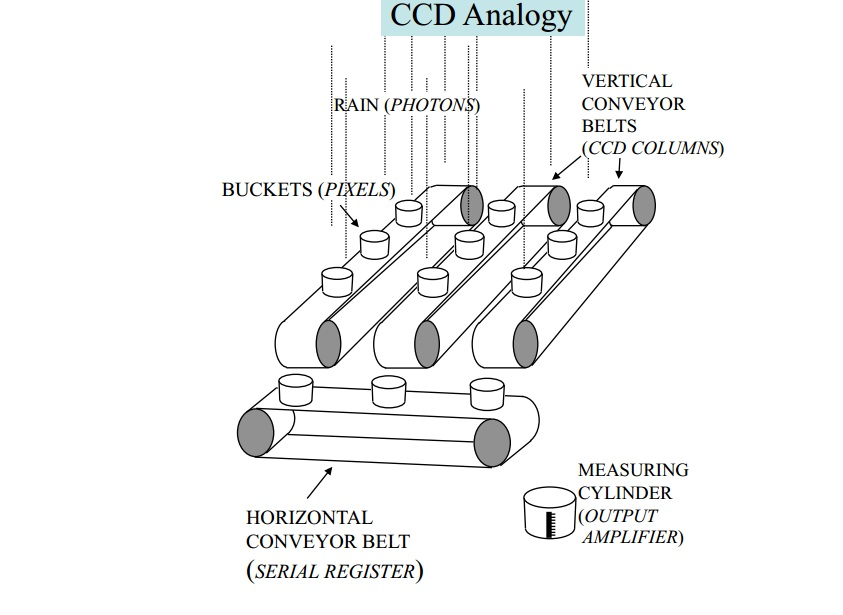
\includegraphics[width=\textwidth]{CCD.jpg}
\end{center}
\caption{Hopefully readout isn't as long as waiting for your luggage on an 
airport conveyor belt.
\label{fig:CCD}}
\end{figure}

\subsection{Adaptive Optics}
Adaptive optics is used to correct wavefront distortions caused by the 
atomsphere using a deformable mirror.  The basic layout is shown below.  Light 
from the telescope is split, with some going to instruments and some going 
to a wavefront sensor that measure the phase errors of the light.  The 
sensor then controls the deformable mirror to match and correct for the 
wavefront errors.  The whole process happens on a timescale faster than 
the time for the wavefront hitting the telescope to change due to changes in 
turbulence.  

\begin{figure}[!h]
\begin{center}
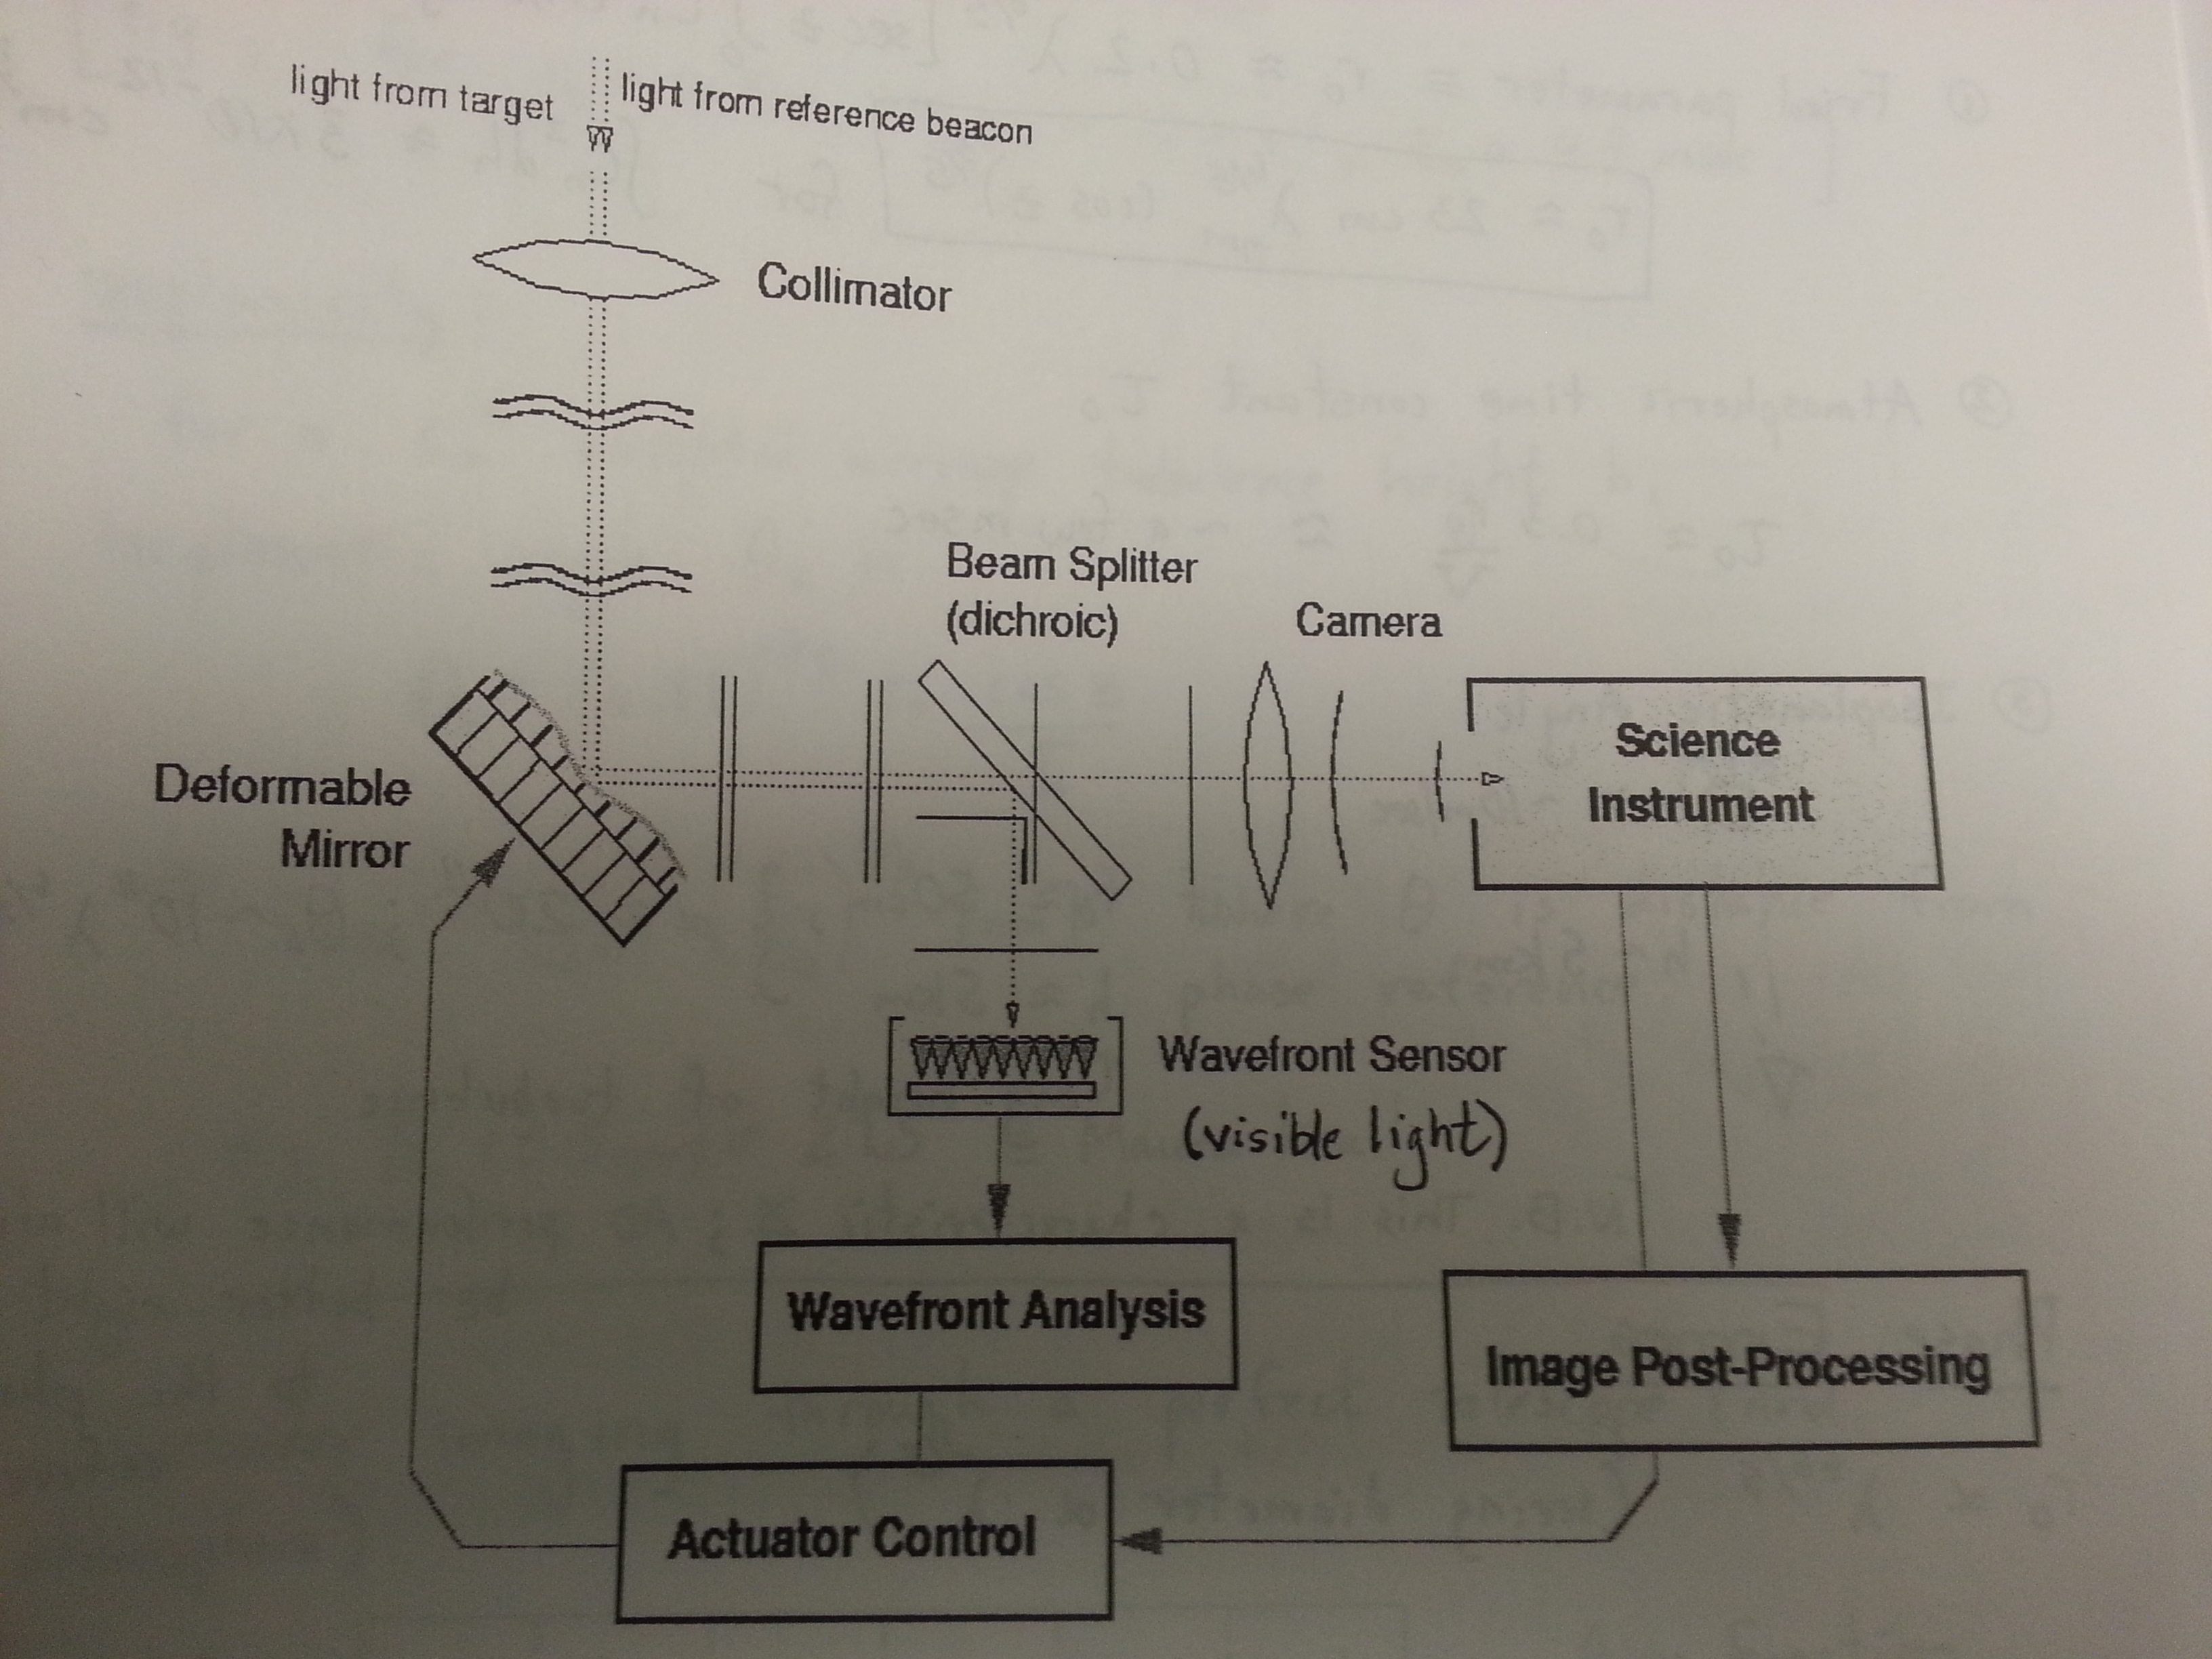
\includegraphics[width=\textwidth]{AO.jpg}
\end{center}
\caption{I'm Shacked and dis-Hartmanned.
\label{fig:AO}}
\end{figure}


